\documentclass[10pt,a4paper]{article}
\usepackage[a4paper]{geometry}
\usepackage[utf8]{inputenc}
\usepackage[english]{babel}
\usepackage{amsmath}
\usepackage{amsfonts}
\usepackage{amssymb}
\usepackage{makeidx}
\usepackage{graphicx}
\usepackage{caption}
\usepackage{subcaption}
\usepackage{color}
\usepackage{import}

\usepackage{multicol}

\usepackage{hyperref}

\usepackage{algorithm2e}

\usepackage{epstopdf}

\usepackage{textpos}

\title{Minimisation par recuit simulée. }
%\author{\href{mailto:matthew.ozon@cpe.fr}{Matthew OZON}} %, \href{mailto:matthew.ozon@cpe.fr}{matthew.ozon@cpe.fr}
\date{}

%begining of the document
\begin{document}
\maketitle

\section*{Énoncé du TP}
Soit la fonction $f$ : 
\begin{align*}
	f &: \mathbb{R} \rightarrow \mathbb{R}\\
	& x \mapsto (x-1.0)(x-0.5)(x-0.3)(x+0.5)
\end{align*}
On souhaite minimiser $f$ en utilisant l'algorithme du recuit simulé en fixant le nombre d’itération à $N=10000$ et en utilisant le noyau de communication qui propose un nouvelle état de la façon suivante : 
\begin{displaymath}
	X\leftarrow X+\delta X \text{ avec } \delta X \sim U([-0.5,0.5])
\end{displaymath}
La variable aléatoire $\delta X$ est définie par une loi uniforme continue sur le segment $[-0.5,0.5]$, donc le cadre théorique impliquant un ensemble discret ne s'applique pas directement, cependant,la génération de nombre aléatoire sur un ordinateur est bien un processus discret, donc on peut appliquer la théorie vue en cours. Caractérisez l'action de la température sur la valeur de sur la valeur du minimum global.


\clearpage

\begin{textblock}{4}(0,-1)
\noindent Nom1 Prénom1\\
Nom2 Prénom2
\end{textblock}

\begin{center}
	\LARGE{Minimisation de fonction non convexe par recuit simulé : influence de la température.}
\end{center}


\section{Introduction/Sujet} (poser le contexte)
Nous cherchons a minimiser la fonction suivante : 
\begin{align*}
	f &: \mathbb{R} \rightarrow \mathbb{R}\\
	& x \mapsto (x-1.0)(x-0.5)(x-0.3)(x+0.5)
\end{align*}
pour cela, nous utilisons un algorithme d'optimisation non convexe : le recuit simulé. Le principe de cette méthode consiste à proposer des solutions aléatoirement et d'accepter toutes les bonnes solutions (celles qui minimisent $f$) mais aussi une fraction contrôlée des mauvaises solutions pour ne pas être bloqué par des minima locaux. De façon plus formelle, voici comme se décompose la méthode : 
\begin{algorithm}[h]
	%\SetAlgoLined
 	%\KwData{this text}
 %\KwResult{how to write algorithm with \LaTeX2e }
	Choisir un état initial $x^{\left(\!0\!\right)}\in\mathbb{R}$ et une température initiale\newline
	\For{n=1 à 10000}{
		$\rho\!\leftarrow\!x^{\left(\!n-1\!\right)}+\delta x$ avec $\delta x \sim U([-0.5,0.5])$ \newline
		\eIf{$f(\rho)\leq f(x^{\left(\!n-1\!\right)})$} 
		{ 
			$x^{\left(\!n\!\right)} \leftarrow \rho$
		}{
			$x^{\left(\!n\!\right)} \leftarrow \rho$ avec la probabilité $e^{\!-\!\frac{\Delta U}{T}}$\
		}
		mettre à jour $T$
	}
	\caption{Recuit simulé pour trouver l'argument du minimum de $f$}
	\label{SA}
\end{algorithm}
\begin{figure}[h]
	\centering
	\scalebox{0.8}{% Title: glps_renderer figure
% Creator: GL2PS 1.3.8, (C) 1999-2012 C. Geuzaine
% For: Octave
% CreationDate: Tue Apr 28 00:28:55 2015
\setlength{\unitlength}{1pt}
\begin{picture}(0,0)
\resizebox{140mm}{70mm}{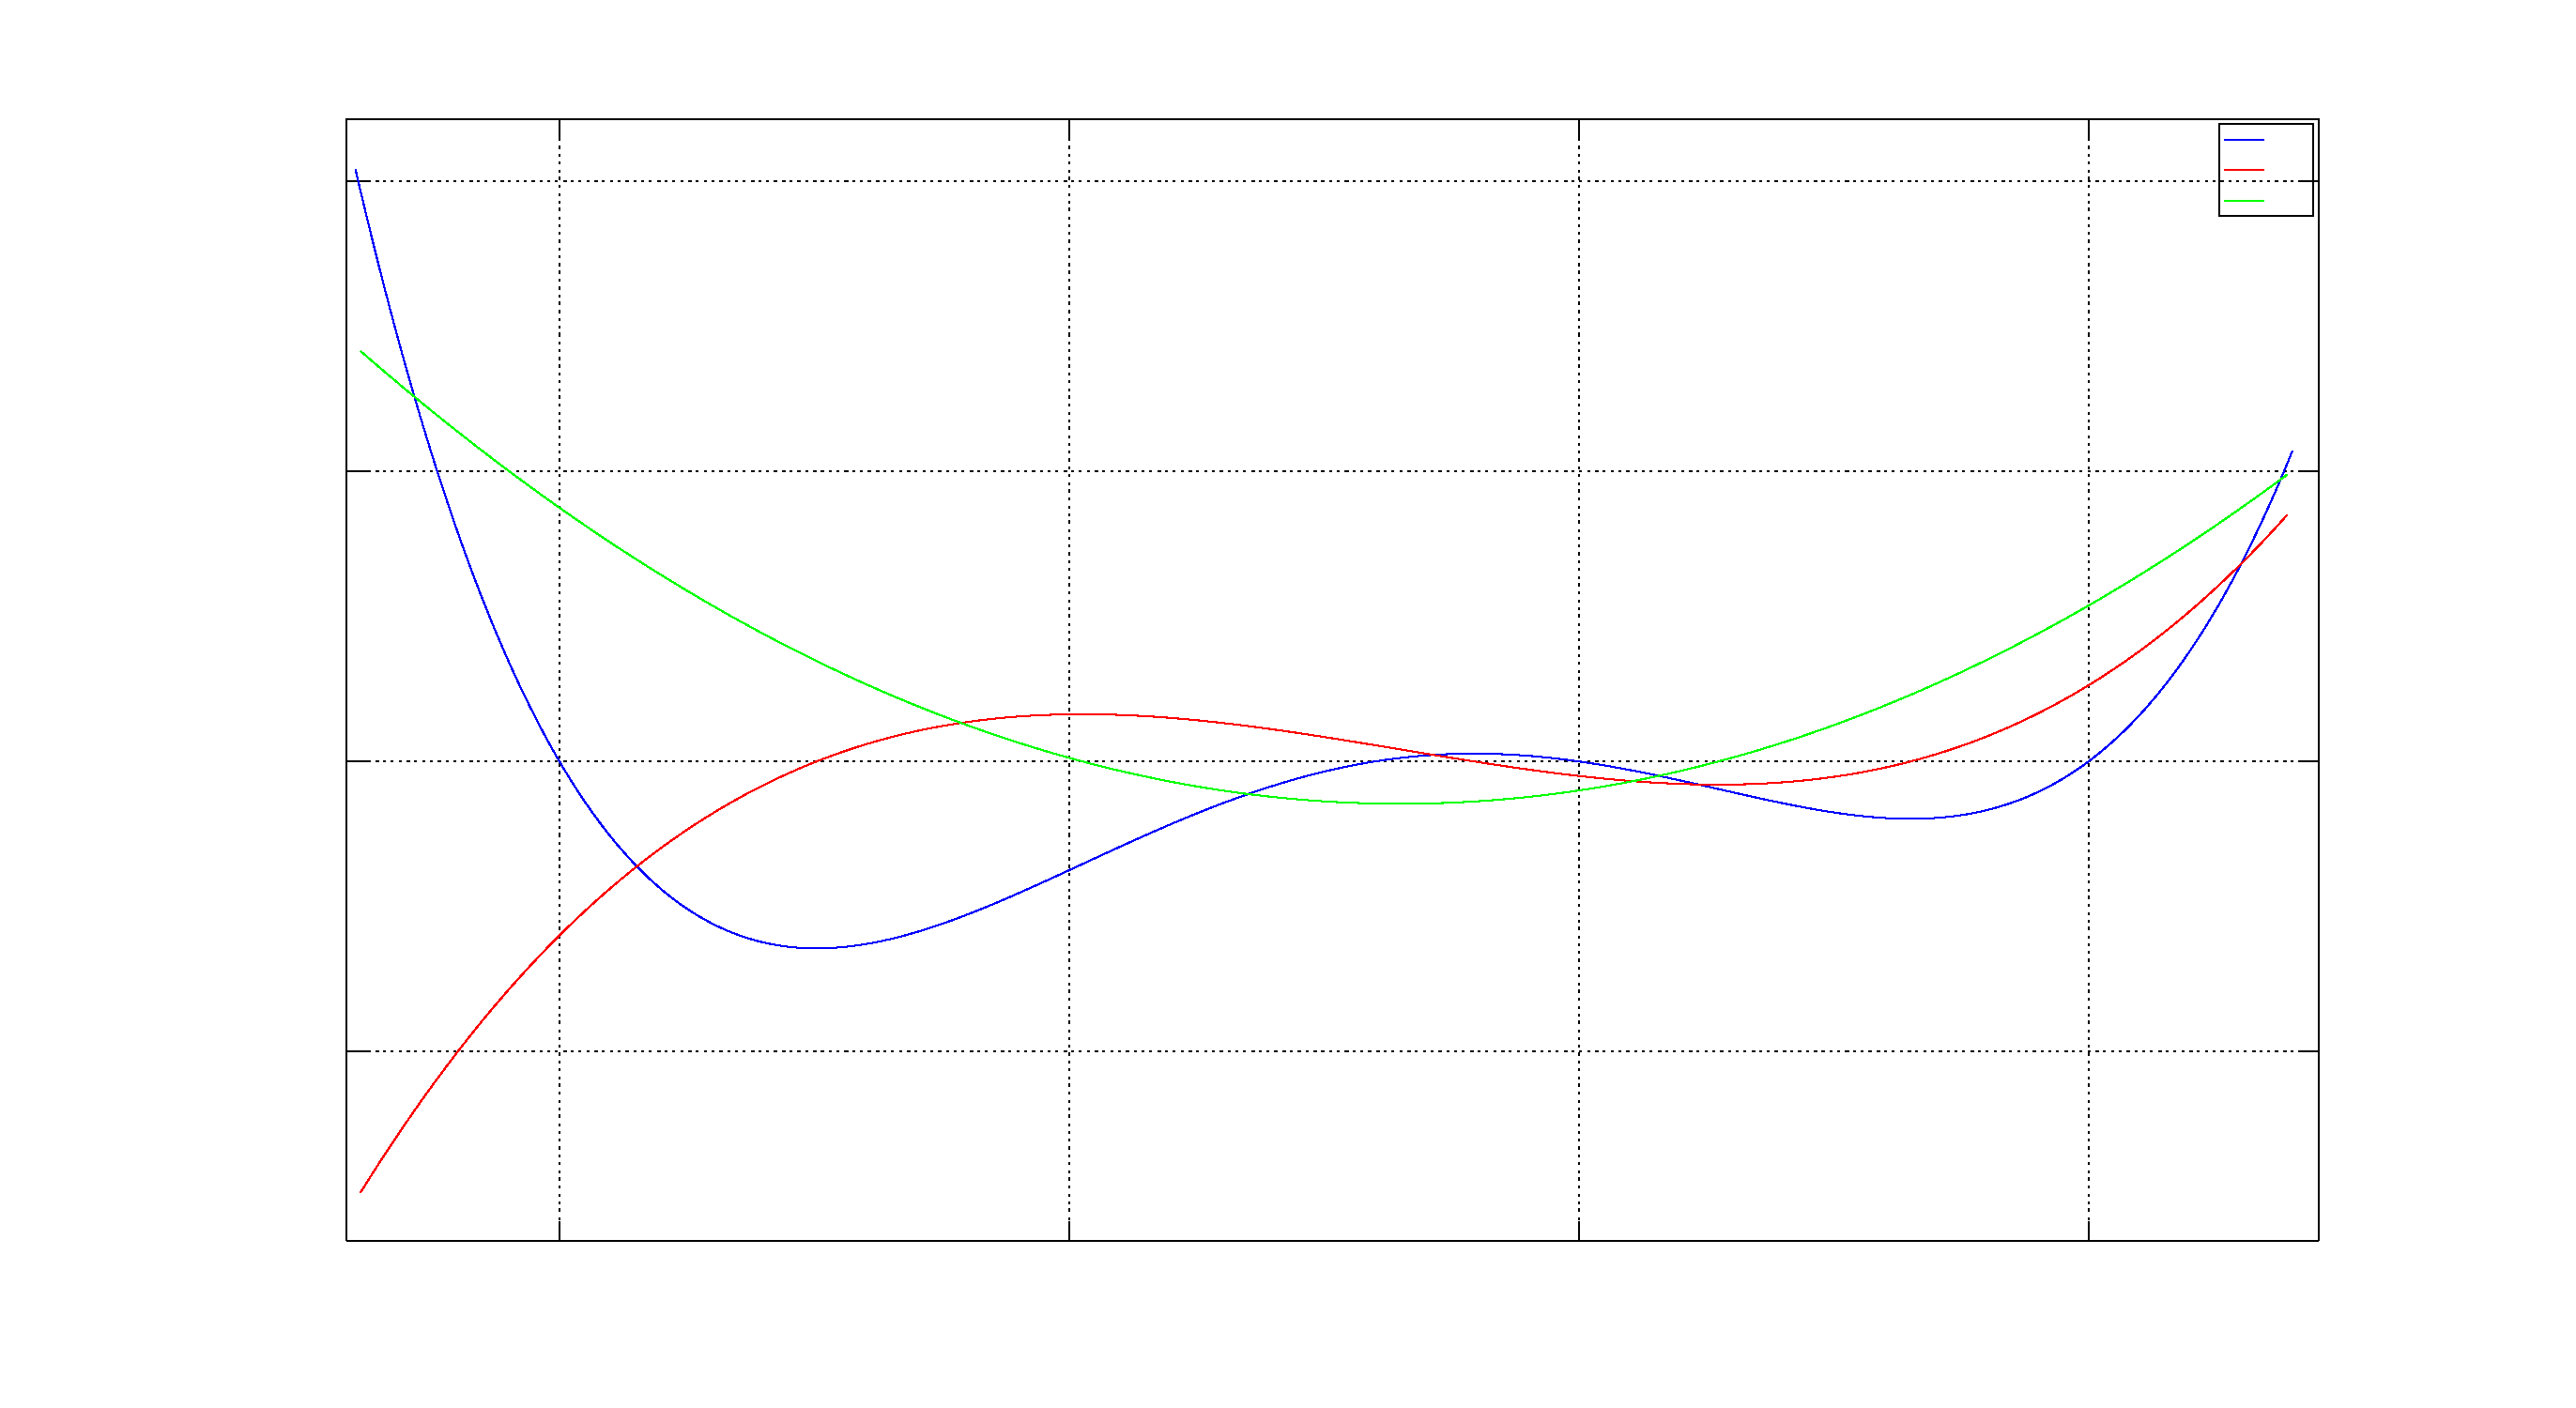
\includegraphics{polynome-inc}}
\end{picture}%
\begin{picture}(360,180)(0,0)
\fontsize{10}{0}
\selectfont\put(84,12){\makebox(0,0)[t]{\textcolor[rgb]{0,0,0}{{-0.5}}}}
\fontsize{10}{0}
\selectfont\put(165,12){\makebox(0,0)[t]{\textcolor[rgb]{0,0,0}{{0}}}}
\fontsize{10}{0}
\selectfont\put(245,12){\makebox(0,0)[t]{\textcolor[rgb]{0,0,0}{{0.5}}}}
\fontsize{10}{0}
\selectfont\put(326,12){\makebox(0,0)[t]{\textcolor[rgb]{0,0,0}{{1}}}}

\fontsize{10}{0}
\selectfont\put(45,49){\makebox(0,0)[r]{\textcolor[rgb]{0,0,0}{{-0.2}}}}
\fontsize{10}{0}
\selectfont\put(45,92){\makebox(0,0)[r]{\textcolor[rgb]{0,0,0}{{0}}}}
\fontsize{10}{0}
\selectfont\put(45,130){\makebox(0,0)[r]{\textcolor[rgb]{0,0,0}{{0.2}}}}
\fontsize{10}{0}
\selectfont\put(45,175){\makebox(0,0)[r]{\textcolor[rgb]{0,0,0}{{0.4}}}}

\fontsize{6}{0}
\selectfont\put(351,182){\makebox(0,0)[l]{\textcolor[rgb]{0,0,0}{{$f$}}}}
\fontsize{6}{0}
\selectfont\put(351,177){\makebox(0,0)[l]{\textcolor[rgb]{0,0,0}{{$f'$}}}}
\fontsize{6}{0}
\selectfont\put(351,172){\makebox(0,0)[l]{\textcolor[rgb]{0,0,0}{{$f''$}}}}
\end{picture}
}
	\caption{Représentation de la fonction (bleue) à minimiser et de ses dérivée (rouge) et dérivée seconde (vert). La dérivée est multipliée par $10$ et la dérivée seconde par $1000$.}
	\label{fonction}
\end{figure}

\section{Expériences/Questions}(si les questions sont clairement formulées, suivez le plan des questions avec la numérotation, sinon, il faut analyser le problème)

Dans un premier temps, nous observons que $f$ a deux minima locaux (dont un est global) et un maximum car $f'$ s'annule trois fois (polynôme de degrés 3) et $f''$ est positive pour deux de ces points, comme illustré sur la figure~\ref{fonction}.
\subsection{Effet de la température}
Pour mettre en évidence les effets de la température sur la recherche (de l'argument) du minimum, nous testons cette algorithme avec plusieurs couples de températures initiales et finales qui correspondent aux niveaux d'acceptations qui sont listés dans le Tableau~\ref{argumentEtTau}
\begin{table}[h] 
	\centering
	\caption{Récapitulatif des arguments des expériences. Chacune est répétée 30 fois et les résultats sont les moyennes des résultats avec leurs écarts-types}
\begin{footnotesize}
   \begin{tabular}{|l|l|l|l|l|l|l|}%8 000 000 000 000 000 000 000
        \hline\vspace{-3mm}
         &  &  & & & \\
        $T_{\text{init}}/T_{\text{fin}}$ & $8.0/10^{-5}$ & $10^{21}/10^{-5}$ & $8.10^{-3}/10^{-5}$ & $8.0/0.1$ & $8.0/10^{-21}$\\\hline
        tau d'acceptation initial   & $0.92\!\pm\!0.02$  &  $1.0\!\pm\!0.0$  &   $0.23\!\pm\!0.03$ &   $0.915\!\pm\!0.03$ &   $0.88\!\pm\!0.03$\\ 
        tau d'acceptation final   & $0.008\!\pm\!0.004$  &  $0.011\!\pm\!0.005$  &   $0.006\!\pm\!0.004$ &   $0.73\!\pm\!0.03$ &   $0.0\!\pm\!0.0$\\ 
        argument      & $-0.248\!\pm\!0.002$    &  $-0.069\!\pm\!0.41$    &   $0.29\!\pm\!0.54$  &   $0.17\!\pm\!0.4$ &   $-0.17\!\pm\!0.27$ \\
        minimum       & $-0.128907\!\pm\!0.00001$  &  $-0.11\!\pm\!0.03$  &   $-0.08\!\pm\!-0.04$ &   $-0.06\!\pm\!0.05$ &   $-0.123\!\pm\!0.022$\\
        \hline
    \end{tabular}
\end{footnotesize}
	\label{argumentEtTau}
\end{table}
On notera, avant toute interprétation, que les tau d'acceptation sont estimés  sur 300 itérations de l'algorithme, ce qui a deux conséquences : la précision des taux est limitée à $\frac{1}{300}$ et la température a le temps d’évoluée ce qui fait aussi evoluer le tau d'acceptation ($e^{\frac{\Delta f}{T}}$).

Dans un premier temps, nous considéreront les températures ``bien choisies'', ce qui veut dire que les tau d'acceptation des mauvaises configurations est au départ dans l'intervalle $[0.6,0.95]$ et à l’arrivée dans $[10^{-5},10^{-3}]$. Nous avons choisie le couple $(8.0/10^{-5})$, qui n'est pas complètement dans le critère énoncé précédemment, cependant l'algorithme converge et il tend vers les bonnes estimations. On observe que la valeur de l'estimation de l'argument minimisant $f$ est précise comparativement aux autres configurations. On peut faire le même commentaire pour la valeur du minimum estimé.

Pour toutes les autres configurations, la valeur de l'argument du minimum est mal estimé, il suffit de comparer ces valeur avec un estimation graphique faire à partir de la figure~\ref{fonction} pour s'en convaincre. (dans ce cas, on peut utiliser le graphique comme argument car il fait office de contre-exemple). En effet, l'algorithme peut se faire piéger dans des bassin d'attraction locaux. Pour les couples $(8.10^{-3}/10^{-5})$,  $(10^{21}/10^{-5})$ et $(8.0/10^{-21})$, la valeur de l'argument du minimum est précisément estimée pour chaque expérience car peu de mauvaise configurations sont acceptées à la fin des itérations. Cependant, la vitesse de décroissance de $T$ n'est pas bien adaptée pour visiter touts les bassins d'attractions, donc, le recuit sort aléatoirement l'un des deux minima. Le couple $(8.0/0.1)$, quant à lui, ne permet pas une bonne estimation car le tau d'acceptation final est trop élevé, donc l'algorithme ne converge pas.


\section{Conclusion/ouverture}
On peut conclure qu'une bonne estimation des températures est une conditions nécessaire pour faire converger le recuit vers un minimum global. Cette conclusion n'est, cependant, valable que pour cet exemple qui ne présente aucun caractère général. Il serait intéressant d’étudier aussi l'influence du nombre d’itération et de la définition du noyau de communication.




\end{document}





\subsection{Effet de l'initialisation}
Pour mettre en valeur les résultats du recuit, nous les avons confrontés aux résultats possible d'une méthode par descente de gradient. Comme on peut le voir sur la figure~\ref{}, la fonction possède deux minimum, et local et un global. En fonction de l'initialisation de la méthode de descente de gradient, le minimum trouver est sot $x_1=$ ou $x_2=$. 




\clearpage

\paragraph{Méthode d'optimisation : } Le recuit est une méthode d'optimisation, ce qui signifie : rechercher les extremum globaux de fonctions.

\paragraph{Le contexte : } le recuit s'utilise sur tout type de fonctions, cependant  les preuves que la méthode fonctionne ne sont que pour les fonctions définies sur des ensembles discrets. Par exemple, on peut définir une fonction $U$ sur un ensemble $\Omega$ discret fini comme $\{0,1\}^N$ avec $N$ la dimension des éléments ($\omega\in\Omega, \omega=\{\omega_n|n\in [\![1,N]\!]\}=\{0,0,1,0,1,1,1,\ldots,0,1,0\}$) : 
\begin{align*}
	U :\quad & \Omega \rightarrow \mathbb{R}\\
	     & \omega \mapsto U(\omega)=\overset{N}{\underset{n=1}{\sum}} f_n(\omega_n) + \overset{N-1}{\underset{n=2}{\sum}} g_n(\omega_{n-1},\omega_{n+1})
\end{align*}
Remarque : la fonction $U$ n'est pas convexe de par sa définition sur un ensemble discret, donc les algorithmes de descente de gradient ne peuvent pas converger vers le(s) extremum globaux

\paragraph{Le recuit simulé : } Cette méthode est différente des méthodes de descente de gradient qui se formulent de la fa\c{}on suivante pour une fonction $f$ différentiable  sur $\mathbb{R}^d$ convexe (au moins localement)
\begin{multicols}{2}
\begin{algorithm}[h]
	%\SetAlgoLined
 	%\KwData{this text}
 %\KwResult{how to write algorithm with \LaTeX2e }
	-initialisation\newline
	$x_0\in\mathbb{R}^d$  point de départ\newline
	$\Delta t$ le pas temporel\newline
	$\delta x = \infty$ critère d'arrêt \newline
	$\epsilon$ la précision du résultat \newline

	-itération\newline
	\While{$\delta x > \epsilon$}{
		incrémente n\newline
		$x_n = x_{n-1} + \Delta t \nabla f (x_{n-1})$
	}
	\caption{Algorithme de descente de gradient}
\end{algorithm}
\end{multicols}

En effet, le but du recuit étant de ne pas se faire piéger par les extremum locaux, une méthode qui ne se fait attirer que pars la plus proche extremum ne pourra pas donner de bon résultats sur des fonctions non convexes. Il faut donc une autre stratégie! Le principale problème des descentes de gradient est qu'elles ne vont que dans un sens (vers l'extrema le plus proche), on va donc autoriser dans une certaine mesure d'aller dans l'autre sens. Bien évidement, on ne va pas accepter d'aller dans le mauvais sens de fa\c{}on anarchique, il va falloir definir comment et dans quelle mesure on va accepter d'aller dans le mauvais sens. Une autre question se pose : comment definir le ``mauvais sens''. Est-ce juste le sens opposé? Non, c'est potentiellement toutes les directions qui mènent a une augmentation de la fonction d'énergie ($U$).

\noindent\emph{Remarque : } le principe du recuit simulé est basé sur la physique statistique dans le cadre de la physique de la matière, donc la fonction à minimiser est souvent appelée : fonction d'énergie.

\paragraph{l'algorithme : } On appel un recuit une chaîne d'état $(\omega_n)_n$ appartenant à $\Omega$ avec la définition des transitions $q$ (probabilité de passage de l'état courant à un autre) et la séquence de température $(T_n)_n$. La chaîne d'états est une chaîne de Markov non homogène qui est générée selon l'algorithme~\ref{SA}.
\begin{algorithm}[h]
	%\SetAlgoLined
 	%\KwData{this text}
 %\KwResult{how to write algorithm with \LaTeX2e }
	Choisir un état initial $\omega^{\left(\!0\!\right)}\in\Omega$\newline
	\For{n=1 à M}{
		choisir un nouvel etat $\rho$ selon $q\!\left(\omega^{\left(\!n-1\!\right)}\!,\!\bullet \right)$\newline
		affecter $\omega^{\left(\!n\!\right)}\!\leftarrow\!\omega^{\left(\!n-1\!\right)}$\newline
		calculer $\Delta U\!\leftarrow\!U\!\!\left(\rho\right)\!-\!U\!\!\left(\omega^{\left(\!n-1\!\right)}\right)$\newline

		on accepte de inconditionnellement les nouveaux états diminuant l'énergie\newline
		\eIf{$\Delta U\leq0$} 
		{ 
			affecter $\omega^{\left(\!n\!\right)} \leftarrow \rho$
		}{
			affecter $\omega^{\left(\!n\!\right)} \leftarrow \rho$ avec la probabilité $e^{\!-\!\frac{\Delta U}{T}}$\
		}
		mettre à jour $T$
	}
	\caption{Recuit simulé pour trouver l'argument du minimum de $U$}
	\label{SA}
\end{algorithm}

\paragraph{Propriété/condition}~\newline

\noindent\emph{Mouvement} La définition des transitions se fait à travers la matrice de probabilité (matrice Markovienne) $q$ qui est une carte des couples $(\omega_1,\omega_2)$ de $\Omega^2$ La matrice $q$ définit donc la probabilité de passer d'un état $\omega_1$ à un état $\omega_2$. Les propriétés de cette matrice sont les suivantes~: 
\begin{itemize}
	\item[1]  $\forall \omega\in\Omega, q(\omega,\bullet)$ est une densite de probabilite sur $\Omega$, donc $\int_{\Omega}q(\omega,\tilde{\omega})\mathrm{d}\tilde{\omega} = 1$
	\item[2]  $q$ est symétrique : il est donc équiprobable de passer de $\omega_1$ à $\omega_2$ que de passer de $\omega_2$ à $\omega_1$.
	\item[3] $q$ est irréductible $\forall (\omega_1,\omega_2)\in \Omega^2$, il existe un chemin $\Gamma=(\omega_n)_{1\leq n \leq K}$ constitué d'éléments de $\Omega$ débutant à $\omega_1$ et finissant à $\omega_2$ tel que $\forall n\in[\![2,K]\!], q(\omega_{n-1},\omega_n)>0$. Ce qui signifie qu'il existe toujours un chemin plus ou moi long pour aller d'un état à un autre : tout état est joignable.
\end{itemize}
\emph{Remarque} : on appel aussi cette matrice le noyau de communication ou noyau de Markov.

\noindent\emph{Transition de la chaîne du recuit} Soit $(X_n)_n$ une suite de variables aléatoires defini par les transition du recuit. On note $P(X_n|X_{n-1})$ la transition d'un état sachant l'état précédent, $P$ est défini comme : 
\begin{displaymath}
	P(X_n=\omega_1|X_{n-1}=\omega_2) = \mathcal{Q}_{T_n}(\omega_1,\omega_2)
\end{displaymath}
avec
\begin{displaymath}
	\mathcal{Q}_{T_n}(\omega_1,\omega_2) = 
	\left\{\begin{array}{cc}
		q(\omega_1,\omega_2) & \text{si } U(\omega_1)<U(\omega_2)\\
		q(\omega_1,\omega_2) e^{-\frac{U(\omega_1)-U(\omega_2)}{T_n}} & \text{si } U(\omega_1)>U(\omega_2)
	\end{array}\right.
\end{displaymath}

\paragraph{Estimation des températures} Il a été prouvé que le recuit converge vers l'un des extremum globaux (de façon équiprobable) en utilisant des schéma de décroissance exponentielle pour la température. La température à l’itération $n\in[\![1,M]\!]$ peut donc s'écrire : 

\begin{displaymath}
	T_n = T_{\text{init}}\left(\frac{T_{\text{fin}}}{T_{\text{init}}}\right)^{\frac{n-1}{M-1}}
\end{displaymath}
Il ne reste donc plus qu'à déterminer $T_{\text{init}}$ et $T_{\text{fin}}$. Pour cela, on écrit le taux moyen d'acceptation des transition qui font augmenter l'énergie. dans un premier temps, on génère une chaîne de  $L$ états $(Y_n)_{1\leq n\leq L}$, en utilisant le noyau de communication $q$, telle que la suite $(\Delta U_n = U(Y_n)-U(Y_{n-1}))_{2\leq n \leq L}$ soit positive pour tous ses termes. Le tau d'acceptation $\chi$ est alors la moyenne des taux d'acceptation
\begin{displaymath}
	\chi = \frac{1}{L-1} \overset{L}{\underset{k=2}{\sum}}e^{\frac{\Delta U_k}{T}}
\end{displaymath}
Ainsi, en définissant $\beta=\frac{1}{T}$ et $f(\beta)=\frac{1}{L-1} \overset{L}{\underset{k=2}{\sum}}e^{\beta\Delta U_k}-\chi$, il est facile de déterminer les températures initiale et finale. En effet, $f$ est strictement monotone par rapport à $\beta$, on peut donc appliquer la méthode de Newton-Raphson pour trouver les zéros de $f$.

\noindent\emph{Remarque} Pour que le recuit fonctionne bien, il faut d'une part un nombre suffisant d'itérations, un bon choix des taux d'acceptations initiale et finale, et un noyau de communication qui convient bien au problème sous-jacent. Le noyau de communication et le nombre d'iteration vont dependre directement du probleme, cependant, les taux d'acceptation sous toujours dans les memes intervalle. Il faut $0<\chi_{\text{fin}}<\!\!<\chi_{\text{init}}<1$, typiquement, $\chi_{\text{init}}\in[0.6,0.9]$ et $\chi_{\text{fin}}\in[10^{-5},10^{-3}]$.



%\subsection{Translation et transpos\'{e}e d'ensemble}


%\begin{displaymath}
%	N_c =  \left|X \odot\left\{ 
%	\begin{array}{|c|c|c|}
%	 \hline 1  & 0  \\
%	 \hline 0  & 0  \\
%	\hline
%	\end{array},
%	\begin{array}{|c|c|c|}
%	 \hline 0  & 1  \\
%	 \hline 1  & 1  \\
%	\hline
%	\end{array}
%\right\}\right|+
%\left|X \odot\left\{ 
%	\begin{array}{|c|c|c|}
%	 \hline 1  & 0  \\
%	 \hline 0  & 1  \\
%	\hline
%	\end{array},
%	\begin{array}{|c|c|c|}
%	 \hline 0  & 1  \\
%	 \hline 1  & 0  \\
%	\hline
%	\end{array}
%\right\}\right|-
%\left|X \odot\left\{ 
%	\begin{array}{|c|c|c|}
%	 \hline 1  & 1  \\
%	 \hline 1  & 0  \\
%	\hline
%	\end{array},
%	\begin{array}{|c|c|c|}
%	 \hline 0  & 0  \\
%	 \hline 0  & 1  \\
%	\hline
%	\end{array}
%\right\}\right|
%\end{displaymath}
%\clearpage
%\subsection{Squelette}
%\begin{displaymath}
%	\mathcal{S}_{B}\left(X\right) = \underset{n\in \mathbb{N}}{\cup} \left(E_{B_n}\left(X\right) \backslash \left(E_{B_n}\left(X\right)\right)\circ B \right)
%\end{displaymath}
%o\`{u} $B_n =\underset{n \text{ fois}}{\underbrace{B\oplus\ldots\oplus B}}$ et par convention $B_0$ est l'ensemble de un pixel \`{a} l'origine. En pratique, on ne fait pas tendre $n$ vers $+\infty$, mais on s'arr\^{e}te quand on atteint idempotence. 

%\clearpage
%
%\begin{verbatim}
%clear all;close all;clc;
%set(gcf,'color','w');%fond blanc
%f=imread('aiguilles_pin.jpg');%\`{a} remplacer par une image de votre choix
%f=f(1:512,1:512);
%[a,b]=size(f);
%subplot(2,2,1);imshow(f);title('image originale');
%f=(f>200);
%whos f
%f=im2double(f);
%subplot(2,2,2);imshow(f);title('image seuill\'{e}e');
%marq=zeros(a,b);% \'{e}quivalent \`{a} : m=zeros(size(f));
%for k=1:10;
%    marq(ceil(a*rand),ceil(b*rand))=1;
%end;
%marq=imdilate(marq,ones(20),'same');
%subplot(2,2,3);imshow(marq);title('marqueur');
%g=imreconstruct(marq,f);
%subplot(2,2,4);imshow(g);title('image reconstruite');
%\end{verbatim}


\end{document}





